\documentclass[UTF8]{ctexart}
\ctexset{section/format=\Large\bfseries}

% Packages


% tikz
\usepackage{tikz}
\usepackage{graphicx}

% listing
\usepackage{listings}
\usepackage{lstfiracode}

% margins
\usepackage{geometry}
\geometry{a4paper, left=3cm,right=3cm,top=2cm,bottom=3cm}

% page header and footer
\usepackage{fancyhdr}
\usepackage{float}
\usepackage{booktabs}
\pagestyle{fancy}
% \rhead{}

% table
\usepackage{tabularx}

% for \FloatBarrier
\usepackage{placeins}

% macros for generating information table
\usepackage{keyval}

\usepackage{hyperref}
\usepackage{lmodern}  % for bold teletype font
\usepackage{amsmath}  % for \hookrightarrow
\usepackage{xcolor}   % for \textcolor


\let\oldparagraph\paragraph
\renewcommand{\paragraph}[1]{\oldparagraph{#1} \mbox{}\\}

\lstset{
	columns=fixed,
	style=FiraCodeStyle,
	numbers=left,
	tabsize=4,
	basicstyle=\small\ttfamily,
	backgroundcolor=\color[RGB]{244,244,244},   % 设定背景颜色:浅晦涩,近透明
	keywordstyle=\color[RGB]{40,40,255},        % 设定关键字颜色
	commentstyle=\color[RGB]{0,96,96},          % 设置代码注释的格式
	stringstyle=\color[RGB]{128,0,0},           % 设置字符串格式
	frame=single,
	breaklines=true,
  	postbreak=\mbox{\textcolor{red}{$\hookrightarrow$}\space},
}

\title{\textbf{DNS隐蔽传输信道}}
\author{李心杨}
\date{2023.04.10}
\begin{document}
	\bibliographystyle{plain}
	\maketitle
	\begin{table}[H]
    \centering
    \begin{tabular}{|p{2.2cm}<{\centering}|p{5cm}<{\centering}|p{2.8cm}<{\centering}|p{2.5cm}<{\centering}|}
    \hline
    \textbf{课程名称} & 网络安全 & \textbf{实验日期} & 2023.04.07 \\ \hline
    \textbf{实验名称} & DNS隐蔽信道传输 & \textbf{实验序号} & 1 \\ \hline
    \textbf{姓名}   & \textbf{学号}   & \textbf{专业}   & \textbf{班级} \\ \hline
	李心杨 & 2020302181022 & 信息安全 & 2020级1班 \\ \hline
    \end{tabular}
    \end{table}
	\tableofcontents
	\pagebreak

	DNS-camo 是一个使用 Rust 编写的项目,它包含了一个 DNS 客户端和一个 DNS 服务器,它们可以使用加密和伪装的 DNS 流量进行通信。它使用 chacha20-poly1305 算法对数据进行加密,并使用 base32 对数据进行编码。加密后的数据被嵌入到 DNS 查询名的前缀或者 DNS 响应中的 IP 地址中。该项目使用预共享密钥进行加密和解密。该项目可以用来绕过防火墙或者审查,访问被封锁的域名或者协议,或者安全和隐秘地传输数据,不引起网络监控的注意。项目源码放在了 \href{https://github.com/xinyangli/dns-camo}{GitHub}上,时间较紧,没有进行进一步的优化,后续可能会继续更新。

	\section{原理阐述}

	\subsection{隐藏字段选择}

	一个DNS请求主要分为5个部分:Header、Question、Answer、Authority、Additional,他们包含的字段及作用如下:

\begin{itemize}
	\item Header:请求头,包含了请求的基本信息,如请求的标识符、操作码、响应码、标志位等。
	\item Question:请求问题,包含了请求的域名、类型和类别。例如,查询www.example.com的A记录,就是一个问题。
	\item Answer:请求答案,包含了请求问题的解析结果,如IP地址、生存时间等。如果请求成功,答案部分至少有一个资源记录。
	\item Authority:请求授权,包含了为请求问题提供权威信息的域名服务器的资源记录。例如,如果请求问题是www.example.com的A记录,授权部分可能包含了example.com域的权威服务器的NS记录和对应的A记录。
	\item Additional:请求附加,包含了与请求问题或答案相关的额外资源记录。例如,如果请求问题是www.example.com的MX记录,附加部分可能包含了邮件服务器的A记录或AAAA记录。
\end{itemize}

\begin{figure}[h]
	\centering
	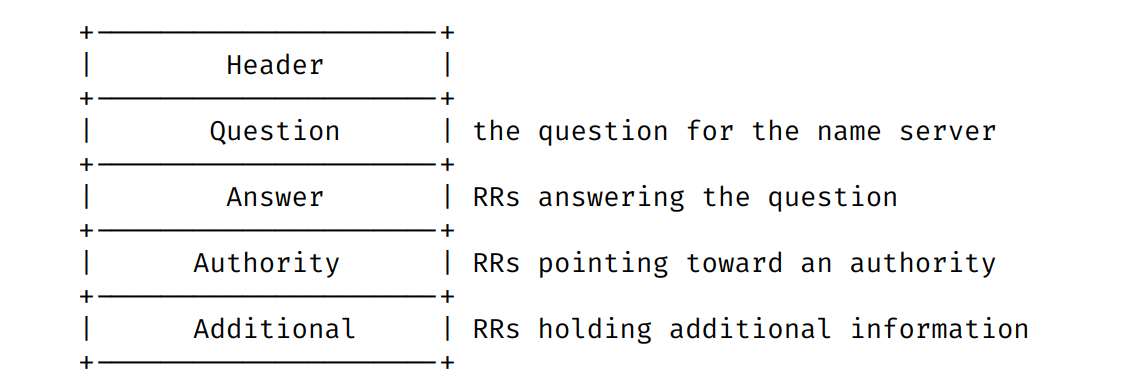
\includegraphics[width=10cm]{images/dns.png}
\end{figure}

	上面的五个部分并不是所有DNS数据包都包含的。对于将信息嵌入在哪里这个问题,其实可以分DNS query和DNS response两种情况来进行讨论。
	
	一般而言,DNS query仅包含Header和Question两个部分,这两个部分中,大部分字段的含义都是确定的,而且Header是固定长度的,非常不利于隐藏信息。想要将信息隐藏在query中,最好的办法实际是将信息放入Question部分的问题中,因为请求的域名是变长的。所以这里我采用的方法是将要传输的数据(加密后)进行base32编码,切分成固定长度后把它们放入一个看似正常的域名的前缀中。比如 s5j19dn.baidu.com,前面的s5j19dn就是我们隐藏的信息。另外,Question部分可以由多个问题组成,所以其实嵌入的信息量仅受UDP数据包大小的限制。

	对于DNS response而言,情况简单很多。首先,DNS response要向客户端返回IP地址(TXT类请求除外),一般情况下,这些IP的可达性并不会被防火墙所侦测,所以我们可以将需要隐藏的信息以二进制的形式存储在IP地址对应的位置。这样的话,每个A类请求可以携带4个字节的数据,每个AAAA类请求可以携带多达16字节的数据。这些返回的数据会被放在Answer和Additional这两个部分中。这是因为,服务端接受到的query中,question的数量是确定的。Answer的数量需要和query对应,不然非常容易被侦测到。但是服务端想要发送的数据不一定恰巧填满所有的Answer,比如,服务端可能需要发送大量数据,但是客户端仅仅询问了一个question。这是,我们将多余的数据以AAAA类请求的形式写入Additional部分,可以最大程度满足服务端传送数据的请求。

	\subsection{加密}

	chacha20-poly1305是一种结合了流密码chacha20和消息认证码poly1305的加密算法,它可以提供高效的数据保密性和完整性。本项目中使用预分享的密钥来对客户端和服务端之间的信息进行加密。

	其实在木马环境中更应该使用非对称加密,因为对称加密的密钥实际上存在于宿主机上,采用逆向分析的方法很容易获取到木马程序使用的密钥,进而对密码发送的消息进行解密,实际上安全性不足。不过这里考虑到对称密码效率高,有成熟地实现,易于使用,且很多网络并不会记录所有流经的数据包,所以即使获取到了密钥也无法获取之前的通信信息,所以还是暂时选择了对称密码的方式来实现demo。

	\section{实现}

	由于最近正在学习rust,所以作为一个练手的项目,整个项目采用rust实现。由于希望通过本次实验了解DNS协议的具体整个项目的核心在Packet这个结构体上,它描述了构建一个DNS请求需要的信息。

\begin{lstlisting}
#[derive(PartialEq, Eq, Debug)]
pub struct Packet {
    header: Header,
    questions: Vec<Question>,
    answers: Vec<Record>,
    authorities: Vec<Record>,
    additional: Vec<Record>,
    is_response: bool,
}
impl Packet {
	fn header_gen(&mut self, id: u16) -> Result<(), DnsParseError>
    pub fn new(request: Option<&Packet>) -> Self;
	pub fn serialize(&mut self, id: u16) -> Result<BitVec<u8, Msb0>, DnsParseError>
	pub fn deserialize<'a, I>(&mut self, mut iter: I) -> Result<(), DnsParseError>
	pub fn embed_data(&mut self, data: &[u8]) -> Result<(), DnsParseError>
	pub fn extract_data(&mut self) -> Vec<u8>
}
\end{lstlisting}

	这个结构体是用来表示一个DNS数据包的,它包含了上面提到的DNS的5个部分,另外还有一个布尔值表示它是不是一个响应数据包。其中,用来在DNS数据包中嵌入和提取数据的是 \lstinline{embed_data} 和 \lstinline{extract_data} 这两个函数。\lstinline{embed_data} 函数接受一个字节数组作为参数,根据数据包是请求还是响应,将数据嵌入到查询名的前缀或者答案的IP地址中。\lstinline{extract_data} 函数从数据包中提取出嵌入的数据,并返回一个字节数组。

	序列化和反序列化是实现中的另一个关键点。它们的作用是将数据在Packet和字节流两种形式中互相转换。实现Packet的序列化和反序列化时,需要先实现其所有子成员的序列化及反序列化。实现时,由于涉及到大小端转换的问题,所以使用用 bitvector 来存储字节流数据。

	加密部分在 Payload 这个结构体中实现,包括读取密钥、生成nonce和加解密等过程。

	\section{测试}

	我使用Docker分别构建了服务端容器和客户端容器,使用docker-compose为这两个容器创建了单独的网络,并完成了容器间通信的测试。

	Dockerfile中,两个容器的命令分别是:

	\begin{lstlisting}[language=bash]
CMD ["/bin/client", "--key=/tmp/key", "--data=186723723", "172.16.238.11", "53"] # 客户端
CMD ["/bin/server", "--key=/tmp/key", "53"] # 服务端
	\end{lstlisting}

	在有docker和docker-compose上的机器上,可以直接使用
	
	\begin{lstlisting}[language=bash]
docker-compose up -d
docker-compose logs --timestamps
	\end{lstlisting}

	来进行测试。测试结果如图~\ref{fig:docker_logs} 所示。图中展示了客户端和服务端打印的log,其中,服务端打印收到的数据的十进制表示方式过程中用到的nonce。

	\begin{figure}[h]
		\centering
		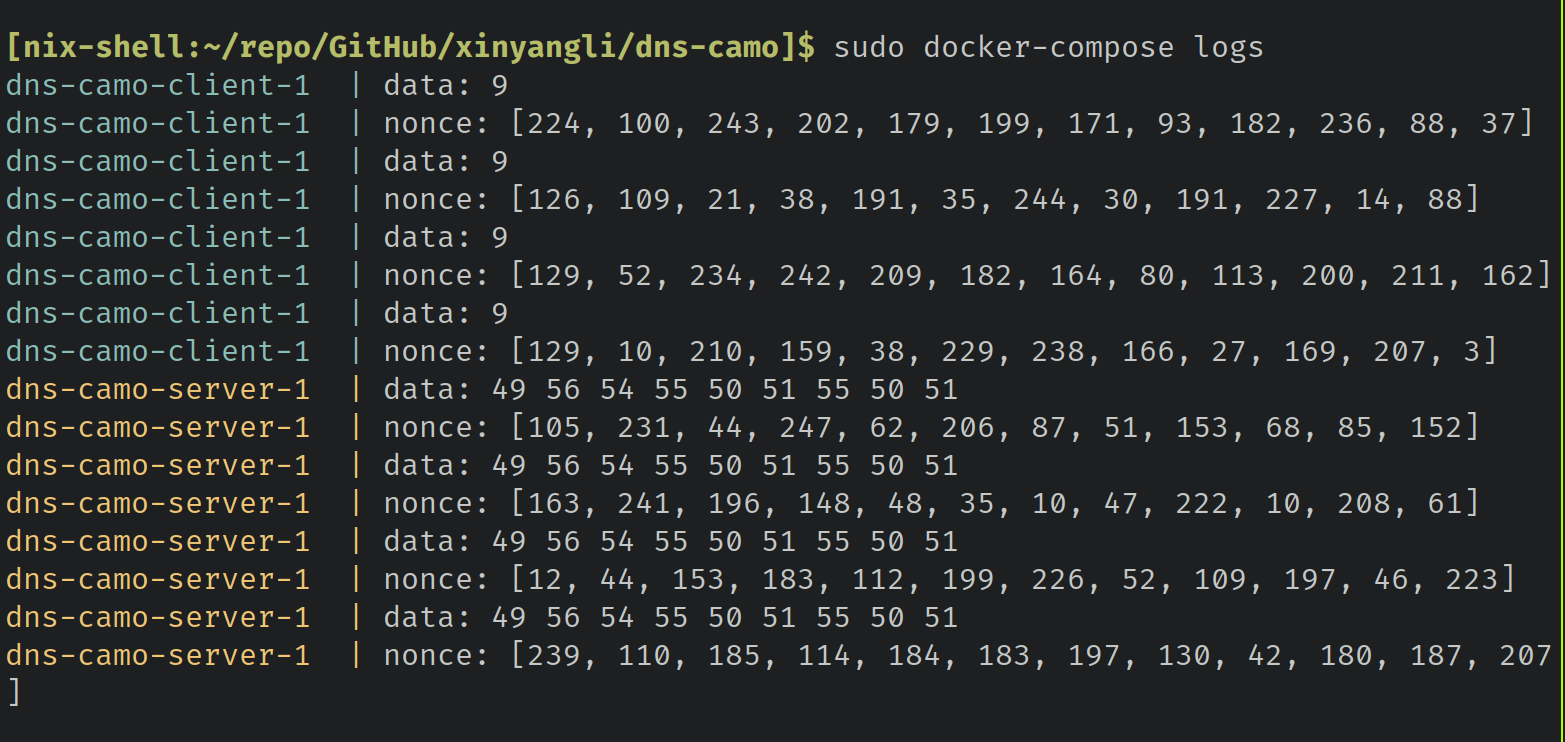
\includegraphics[width=12cm]{images/docker_logs.png}
		\caption{\lstinline{docker-compose logs} 的结果}
		\label{fig:docker_logs}
	\end{figure}
	
	使用Wireshark对我们使用docker-compose创建的网桥进行抓包,进一步验证其中传输数据的格式是否符合DNS标准。抓包的结果如图\ref{fig:wireshark} 所示。从结果中我们可以看到,数据包是按照一去一回的方式传送的。

	\begin{figure}[h]
		\centering
		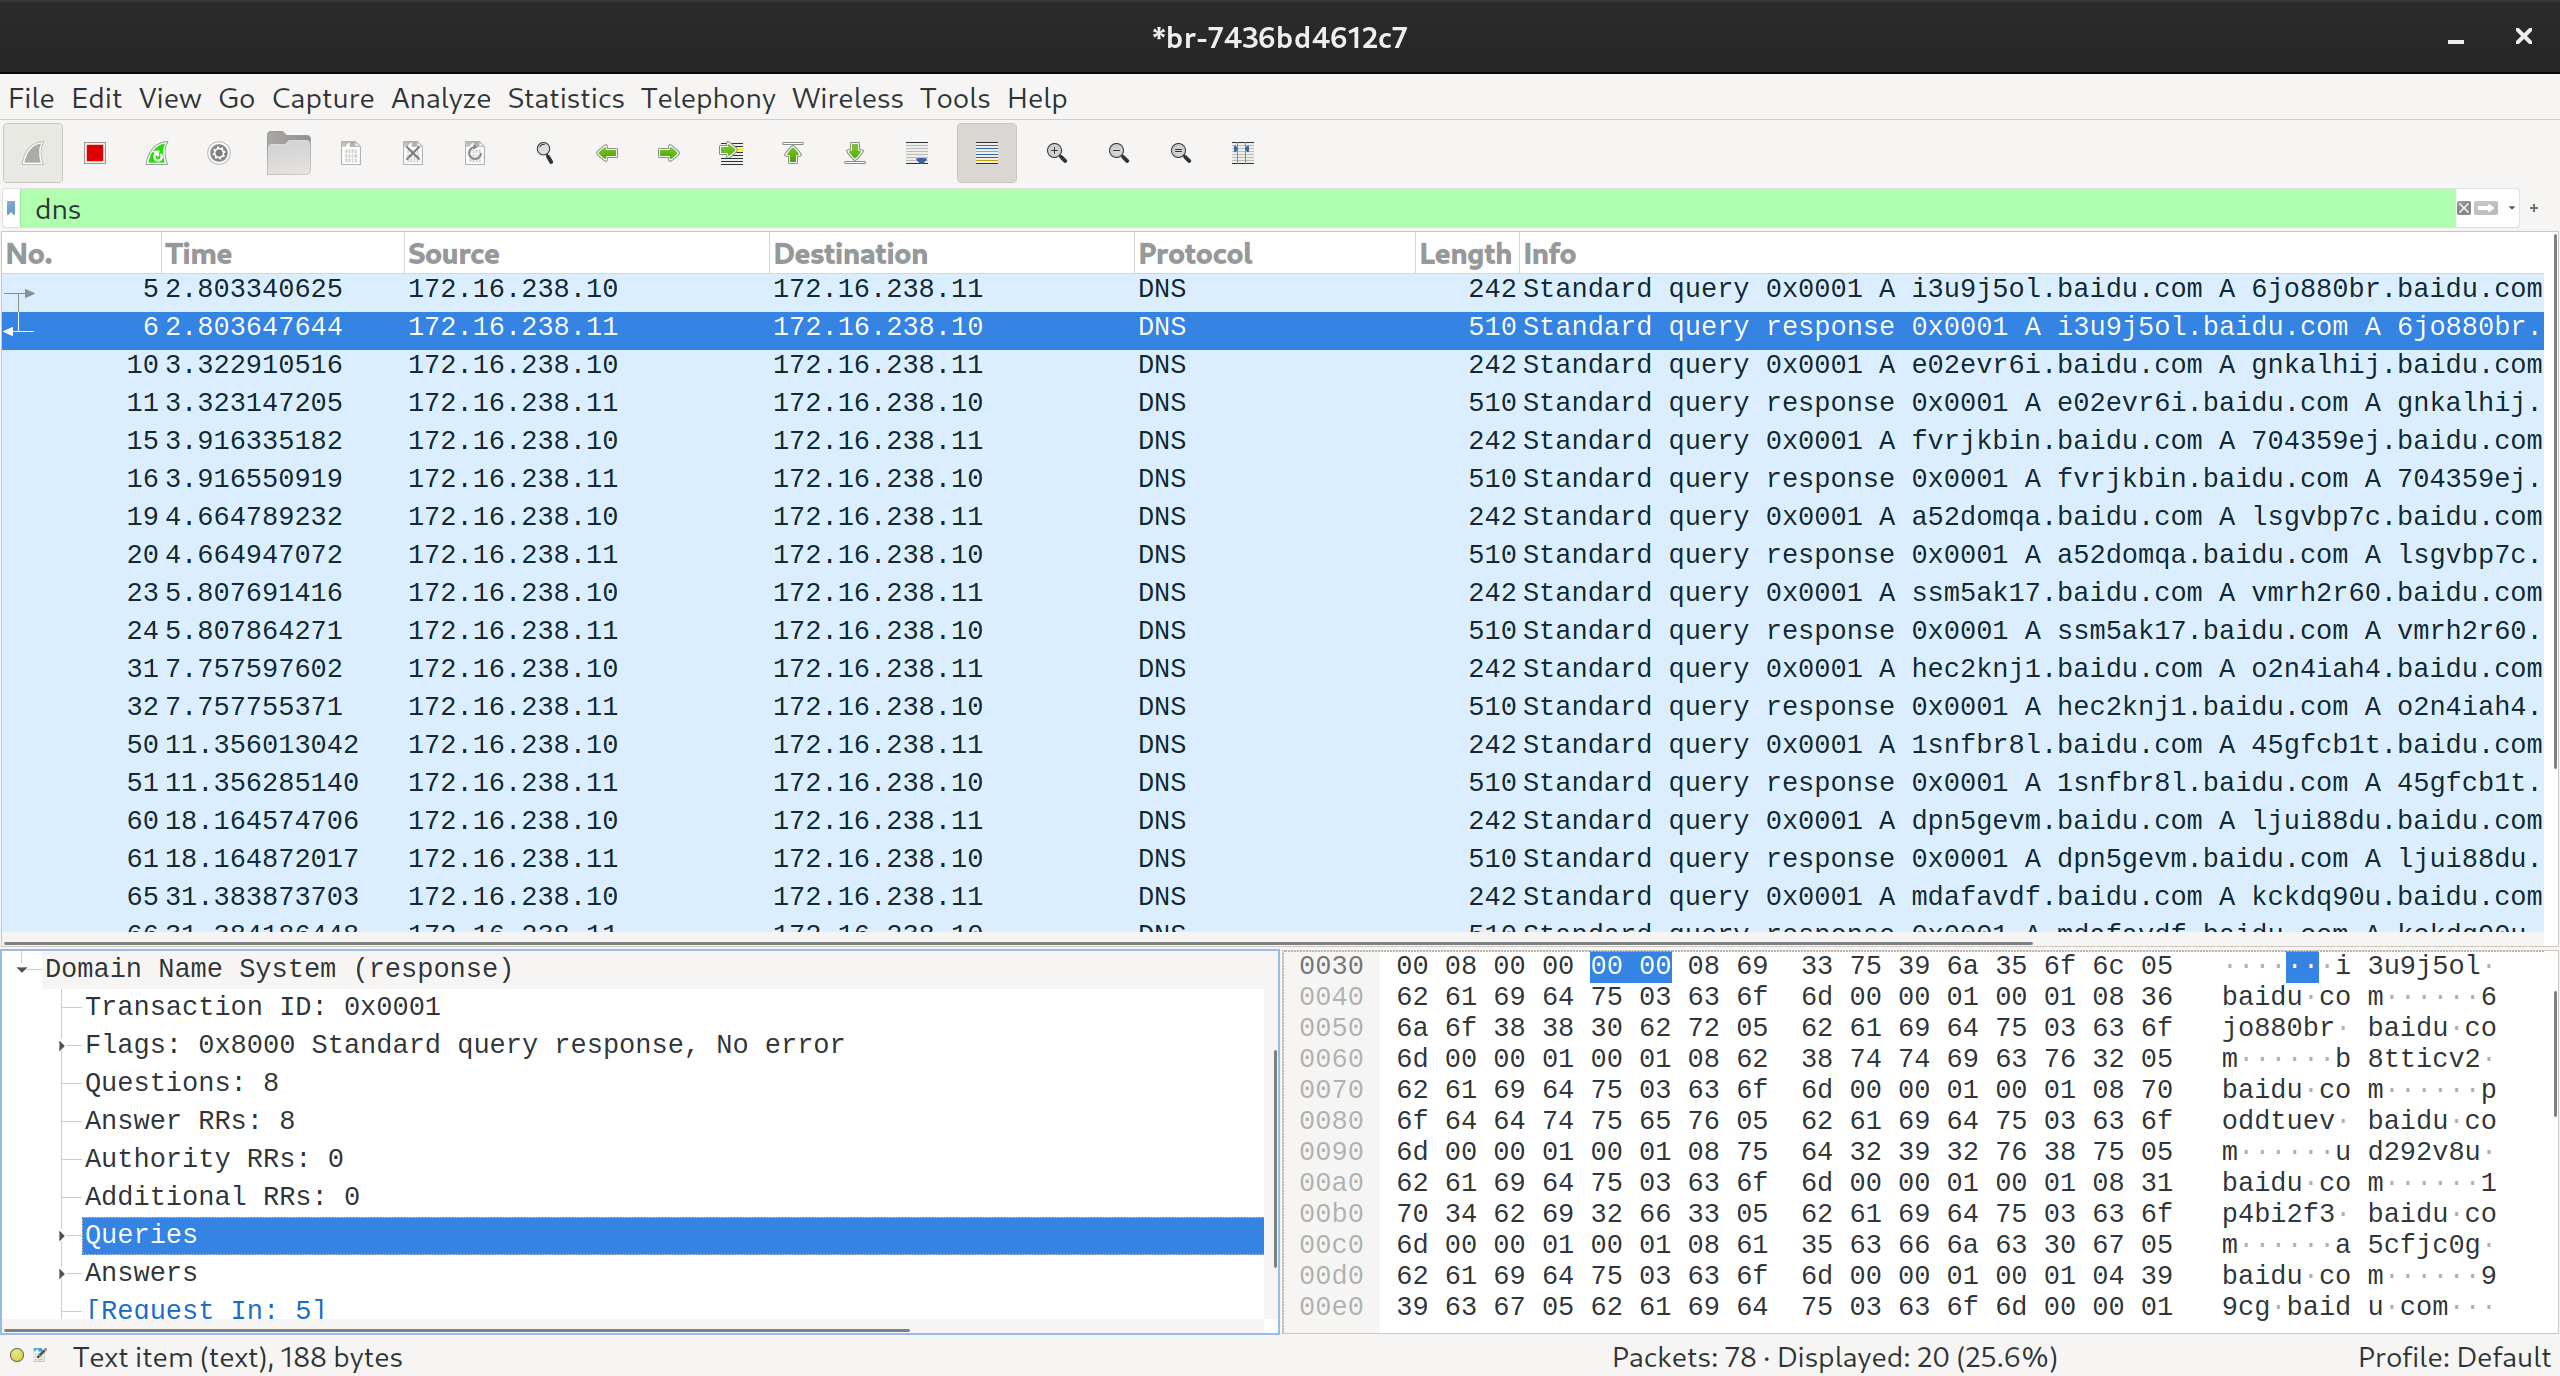
\includegraphics[width=12cm]{images/wireshark.png}
		\caption{wireshark 抓包结果}
		\label{fig:wireshark}
	\end{figure}

	\section{项目总结}

	由于项目时间较紧,所以仍有很多不完善的地方。比如在DNS reponse嵌入时,IPv4和IPv6的长度都是固定的,如何在数据分组后对齐的问题就没有处理完善,现在遇到nonce中含有后缀0的情况仍会出错。之后会继续进行修复和完善。

	不过这是我第一次通篇阅读RFC文档,看起来很冗长的RFC文档其实结构清晰,通过目录可以很方便的找到需要的部分。

\end{document}
